
\subsection{Feature Extraction}\label{chp3-subsec3}
Reviewing the literature, one can observe that some features are used more widely than others, such as color and shape characteristics. 
This is due to the fact that computerized systems are developed to mimic dermatologists' assessment, by using the discriminative characteristics defined in the clinical ``ABCD'' rule for instance.
Thus, we also incorporate some common shape and color descriptors along with texture features.
Shape features ($S$), color statistics and histograms ($C_{1}$), and \ac{glcm} features ($T_{2}$) are chosen because they were used widely in the past.
However, the rest of the descriptors, such as the Opponent Color Space ($C_{2}$), color intensities ($C_{3}$), \ac{lbp} ($T_{1}$), Gabor Filter ($T_{3}$), \ac{hog} ($T_{4}$), and $SIFT$ ($T_{5}$) are chosen because they are efficient and well established color and texture descriptors and have barely been used for the detection of melanoma.
These features are summarized in Table~\ref{Tab:Table2} and explained in the following.

%\input{Chapter3/Figure4.tex}	
%%\begin{table}	
%\resizebox{0.9\textwidth}{0.49\textheight}{
%    \small{
%\begin{longtable}{|p{0.24\textwidth}|p{0.5\textwidth}}
	\begin{longtable}{lc}
	\caption[Extracted features by \ac{glcm} descriptor]{The list of \ac{glcm} statistics ($f_{1}$--$f_{22}$)~\cite{haralick1973textural,clausi2002analysis,soh1999texture} used in our experiments.
	The first section of the table represents the primary measures derived from the co-occurrence matrix $C_{ij}$ for calculating the features.
	Here, $\mu_{x}$, $\mu_{y}$, $\sigma_{x}$, and $\sigma_{y}$ are the mean and standard deviation of $C_{ij}$ with respect to $i$ and $j$, respectively.
	$H_{x}$ and $H_{y}$ are entropy of $C_{x}$ and $C_{y}$}\\
%\begin{center}	
	\toprule
	Co-occurrence matrix & $C_{ij} = P_{ij}/\sum_{i,j=1}^{G} P_{ij}$\\
	& \\[-0.8ex]	
	$C_{x}(i)$ & $\sum_{j=1}^{G}C_{ij}$\\
	& \\[-0.8ex]	
	$C_{y}(j)$ & $\sum_{i=1}^{G}C_{ij}$\\
	& \\[-0.8ex]	
	$C_{x+y}(k)$ & $\sum_{{ij}_{i+j=k}} C_{ij}, k = 2,3 , 2G$ \\
	& \\[-0.8ex]	
	$C_{x-y}(k)$ & $\sum_{{ij}_{|i-j|=k}} C_{ij}, k = 0,1 , G-1$ \\	
	& \\[-0.8ex]	
	$H_{xy}$ & $-\sum_{ij}C_{ij}\log C_{ij}$ \\	
	& \\[-0.8ex]	
	$H_{xy1}$ & $-\sum_{ij}C_{ij}\log(C_{x}(i)C_{y}(j))$\\
	& \\[-0.8ex]	
	$H_{xy2}$ & $-\sum_{ij}C_{x}(i)C_{y}(j)\log(C_{x}(i)C_{y}(j))$\\
	& \\[-0.8ex]	
	\hdashline	
	& \\[-0.8ex]		
	$f_{1}$: Maximum probability & $\max\{C_{ij} , \forall (ij)\}$ \\
	& \\[-0.8ex]
	$f_{2}$: Uniformity & $\sum_{ij} C_{ij}^{2}$ \\
	& \\[-0.8ex]
	$f_{3}$: Entropy & $\sum_{ij}C_{ij}\log C_{ij}$\\
	& \\[-0.8ex]
	$f_{4}$: Dissimilarity & $\sum_{ij} C_{ij}|i-j|$\\
	& \\[-0.8ex]
	$f_{5}$: Contrast & $\sum_{ij}C_{ij}|i-j|^{2}$ \\
	& \\[-1ex]
	$f_{6}$: Inverse difference & $\sum_{ij}C_{ij}/(1+|i-j|)$ \\
	&  \\[-1ex]
	$f_{7}$: Inverse difference moment & $\sum_{ij}C_{ij}/(1+|i-j|^{2})$ \\
	
%	\hline
%	\pagebreak
%	\hline
	& \\[-1ex]
	$f_{8}$: Correlation~1 & $\sum_{ij}(i-\mu_{x})(j-\mu_{y})C_{ij}/(\sigma_{x}\sigma_{y})$\\
	& \\[-1ex] 	
	$f_{9}$: Inverse difference normalized & $\sum_{ij}C_{ij}/(1+|i-j|/N)$\\
	& \\[-1ex]
	$f_{10}$: Sum of squares & $\sum_{ij} (i-\mu)^{2}C_{ij}$ \\
	& \\[-1ex]				
	$f_{11}$: Inverse difference moment normalized & $\sum_{ij}C_{ij}/(1+|i-j|^{2}/N^{2})$\\
	& \\[-1ex]
	$f_{12}$: Sum of average & $\sum_{i=1}^{2N-1}(i+1)C_{x+y}(i)$\\
	& \\[-1ex]
	$f_{13}$: Sum entropy & $S_{e} = -\sum_{i=1}^{2N-1}C_{x+y}(i)\log C_{x+y}(i)$\\
	& \\[-1ex]
	$f_{14}$: Sum variance & $\sum_{i=1}^{2N-1}(i+1-S_{e})^{2}C_{x+y}(i)$\\
	& \\[-1ex]
	$f_{15}$: Difference variance & $\sum_{i=1}^{2N-1}i^{2}C_{x-y}(i+1)$\\
	& \\[-1ex]
	$f_{16}$: Difference entropy & $-\sum_{i=1}^{2N-1} C_{x-y}(i+1)\log C_{x-y}(i)$\\
	& \\[-1ex]
	$f_{17}$: Information measure of correlation~1 & $H_{xy}-H_{xy1}/\max(H_{x},H_{y})$ \\
	& \\[-1ex]
	$f_{18}$: Information measure of correlation~2 & $\sqrt{1-e^{-2(H_{xy2}-H_{xy})}}$\\
	& \\[-1ex]
	$f_{19}$: Auto correlation & $C = \sum_{ij}ijC_{ij}$\\
	& \\[-1ex]	
%	\hline
%	\pagebreak
%	\hline
	$f_{20}$: Correlation~2 &  $(AC-\mu_{x}\mu_{y})/\sigma_{x}\sigma_{y}$ \\
	& \\[-1ex]	
	$f_{21}$: Cluster shade & $\sum_{ij} (i+j-\mu_{x}-\mu_{y})^{3}C_{ij}$\\
	& \\[-1ex]	
	$f_{22}$: Cluster prominence & $\sum_{ij} (i+j-\mu_{x}-\mu_{y})^{4}C_{ij}$\\
	\bottomrule
	\label{tab:glcmfeatures}
  	\end{longtable}
%}
%    }
%	\end{center}
%\label{Tab:glcmfeatures}
%\end{table}

\begin{description}
\item[Shape ($S$)] features were created with reference to \cite{maglogiannis2009overview}.
This group of descriptors measures the thinness ratio, border asymmetry, distance variance of border points to the center and statistics (minimum, maximum, average and variance) of the gradient operator along the lesion's border.
	The thinness ratio measures the circularity of a lesion: $TR = 4\pi Area / Perimeter^2$. 
	And border asymmetry computes the percent of non-overlapping areas after a hypothetical folding of the lesion around its greatest diameter. 
\item[Color Variance and Color Histogram ($C_{1}$)] is a feature descriptor that has been widely used in the past for the detection of melanoma.
This descriptor contains the mean and variance of nine color channels ($R,G,B, H,S,V, L^*,a^*,b^*$) and histograms for $R$, $G$ and $B$ channels.
Each histogram is constructed with $42$ bins, leading to a final descriptor of size $(9\times2)+(42\times3) = 144$.
\end{description}
\begin{description}
\item[Opponent Color Space Angle and Hue Histogram ($C_{2}$)] were first proposed in \cite{van2006coloring} as local color features.
These descriptors were chosen due to their robustness to photometric (shadow, shading, specularities and changes of the light source) and geometrical (viewpoint, zoom and object orientation) variation.
These rotation invariant and robust descriptors are derived from $RGB$ channels using the following equations: 

\begin{subequations}
\begin{align}
	\begin{pmatrix}
	\mathcal{O}_{1}\\\mathcal{O}_{2} \\\mathcal{O}_{3}
	\end{pmatrix} & =
	\begin{pmatrix}
	(R-G)/\sqrt{2}\\
	(R+G-2B)/\sqrt{6}\\
	(R+G+B)/\sqrt{3}
	\end{pmatrix}~, \label{eq:opponent}\\	 
	H^{\mathcal{O}} & = \arctan\left(\frac{\sqrt{3}(R-G)}{R+G-2B}\right)~,\\
	\theta_{d}^{\mathcal{O}} & = \arctan\left(\frac{\sqrt{3}(R'_{d}-G'_{d})}{R'_{d}+G'_{d}-2B'_{d}}\right)~,	
\end{align}
\label{eq:HueOppAngle}
\end{subequations}	
\noindent Here $d$ denotes the spatial coordinates of ($x$,$y$) and $R'_{d}$, $G'_{d}$, $B'_{d}$ denote the first order derivatives of $RGB$ with respect to the coordinates.
This color descriptor is built by taking a 42 bins histogram for the opponent angle $\theta^{O}_{d}$ and the hue channel $H^{\mathcal{O}}$, for a final descriptor size of 84 dimensions.

%\item[Color intensities ($C_{3}$)] represent the color information in a simplest form, their intensities.
\item[Color intensities ($C_{3}$)] represent the color information in its simplest form---their intensities.
This descriptor concatenates color intensities in $R$, $G$ and $B$ to create a feature descriptor.
\item[\acf{clbp} ($T_{1}$)] is a discriminative rotation invariant feature descriptor proposed by Guo~et al.~\cite{guo2010completed}.
\ac{clbp} is a completed version of \ac{lbp}~\cite{ojala2002multiresolution}, especially designed for texture classification.
In both descriptors, a central pixel ($g_c$) in a neighborhood defined by radius $R$ is compared to its neighborhood pixels ($g_{p}$, at distance $R$ from the central pixel) and their differences are encoded in terms of binary patterns.
The binary patterns are calculated for each pixel in a given image and their histogram defines the final descriptor.
\newcounter{row}
\newcounter{col}
\newcommand\setrow[3]{
  \setcounter{col}{1}
  \foreach \n in {#1, #2, #3} {
    \edef\x{\value{col} - 0.5}
    \edef\y{3.5 - \value{row}}
    \node[anchor=center] at (\x, \y) {\n};
    \stepcounter{col}
  }
  \stepcounter{row}
}

%  
\tikzstyle{module}=[draw, draw=blue!80, text width=10em, 
    text centered, minimum height=5em, minimum width = 15em, drop shadow, rounded corners,
    fill=blue!30]
    
\tikzstyle{block} = [rectangle, draw, fill=blue!30, 
     text width=5em,text centered, rounded corners, minimum height=4em, minimum width = 5em]
\tikzstyle{block1} = [rectangle, draw, fill=white!20, 
     text width=5em,text centered, rounded corners, minimum height=4em, minimum width = 5em]

\tikzstyle{line} = [draw, -latex']

% Define distances for bordering
\def\blockdist{1}
\def\edgedist{1.5}
  
\begin{figure}			
\begin{center}
\subfloat[]{
\scalefont{0.7}
\begin{tikzpicture}[scale=.7]

  \begin{scope}
    \draw (0, 0) grid (3, 3);
    \draw[very thick, scale=3] (0, 0) grid (1, 1);

    \setcounter{row}{1}
    \setrow {9}{12}{34} 
    \setrow {10}{\textbf{25}}{28}  
    \setrow {99}{64}{56}  
    \node[anchor=center] at (1.5, -0.5) {Original Image};
  \end{scope}

  \begin{scope}[xshift=4cm]
    \draw (0, 0) grid (3,3);
    \draw[very thick, scale=3] (0, 0) grid (1,1);

    \setcounter{row}{1}
    \setrow {-16}{-13}{9}  
    \setrow {-15}{0}{3}  
    \setrow {74}{39}{31} 
    \node[anchor=center] at (1.5, -0.5) {Local Difference};
  \end{scope}

  \begin{scope}[yshift=-4cm]
    \draw (0, 0) grid (3,3);
    \draw[very thick, scale=3] (0, 0) grid (1,1);

    \setcounter{row}{1}
    \setrow {-1}{-1}{1}  
    \setrow {-1}{}{1}  
    \setrow {1}{1}{1} 
    \node[anchor=center] at (1.5, -0.5) {Sign Component};
  \end{scope}
  
    \begin{scope}[yshift=-4cm,xshift =4cm]
    \draw (0, 0) grid (3,3);
    \draw[very thick, scale=3] (0, 0) grid (1,1);

    \setcounter{row}{1}
    \setrow {16}{13}{9}  
    \setrow {15}{}{3}  
    \setrow {74}{39}{31} 
    \node[anchor=center] at (1.5, -0.5) {Magnitude Component};
  \end{scope}
\end{tikzpicture}
}\\
\subfloat[]{
\begin{tikzpicture}[node distance = 10cm,scale=0.7, every node/.style={scale=0.7}] % 
    % Place nodes   
\begin{scope}[node distance=10cm]
	\node[block] (CLBPs){ $CLBP_{s}$};
\end{scope}
\node[block,below of=CLBPs , node distance = 3cm] (CLBPm) { $CLBP_{m}$};
\node[block,below of=CLBPm, node distance =3cm] (CLBPc) { $CLBP_{c}$};
\node [block, left of=CLBPc, node distance =4cm] (GL) {Grey level of center};
\node [block, above of=GL, node distance =4cm] (LC) {Local Differences}; 
    
    \begin{pgfonlayer}{background}
	\path (LC.west |- LC.north)+(-0.3,-0.8+\blockdist) node (a) {};
    \path (GL.east |- GL.south)+(+0.3,-0.3) node (b) {};          
    \path[fill=blue!10,rounded corners, draw=blue!20, dashed] (a) rectangle (b);
	\end{pgfonlayer}
	
	\begin{pgfonlayer}{background}
	\path (CLBPs.west |- CLBPs.north)+(-0.3,-0.3+\blockdist) node (c) {};
    \path (CLBPc.east |- CLBPc.south)+(+0.3,-0.3) node (d) {};          
    \path[fill=blue!10,rounded corners, draw=blue!20, dashed] (c) rectangle (d);
	\end{pgfonlayer}
	\path (CLBPs.west |- CLBPs.north) +(+1.05,-0.7+\blockdist) node (bgfea) { Binary Patterns};
	
	\path (CLBPs.east |- CLBPs.north)+(0.2,-0.4+\blockdist) node (i) {};
	\path (CLBPc.east |- CLBPc.south)+(0.2,-0.4) node (j) {};

	\draw[decorate,decoration={brace,raise=6pt,amplitude=10pt}, thick]
    (i)--(j) ;
    
    	\path (CLBPs.west |- CLBPs.north)+(-0.15,0) node (k) {};
	\path (CLBPm.west |- CLBPm.south)+(-0.15,0) node (l) {};
text width=3cm
	\draw[decorate,decoration={brace,raise=6pt,amplitude=10pt, mirror}, thick]
    (k)--(l) ;
    
	%% Defining a position for the next block
	\path (CLBPm.east |- CLBPm.north)+(+0.5,-0.6) node (e) {};
	\node[block,right of=CLBPm, node distance = 4.5cm] (CLBPMap) {CLBP Map};
	\node[block,right of=CLBPMap, node distance = 3cm] (CLBPHist) {CLBP \\ Histogram};

	\path (LC.west |- LC.south)+(+0.5,-1) node (f) {};
	\node[block1,left of=f, node distance = +3cm] (Img) {Original \\ Image};
	\path (LC.west |- LC.north)+(-0.15,0) node (m) {};
	\path (GL.west |- GL.south)+(-0.15,0) node (n) {};
		\draw[decorate,decoration={brace,raise=6pt,amplitude=10pt, mirror}, thick]
    (m)--(n) ;
    
    \path [line] (CLBPMap) -- (CLBPHist);
    \path (CLBPm.east |- CLBPm.south)+(1.1,0.7) node (o) {};
    \path [line] (o)--(CLBPMap); 

\end{tikzpicture}}
\end{center}
\caption[\ac{clbp} algorithm]{\ac{clbp} descriptor process. An example of how local distances, sign and magnitude components are calculated is given in (a), while (b) shows an overall view of the CLBP process.}
\label{fig:CLBPFig}
\end{figure}

\begin{figure}
\centering
\subfloat[$\pi/6$]{

\includegraphics[scale=0.06]{Chapter3/Figures/Gabor-pi-6.png}}
\subfloat[$\pi/3$]{

\includegraphics[scale=0.06]{Chapter3/Figures/Gabor-pi-3.png}}
\subfloat[$\pi/2$]{
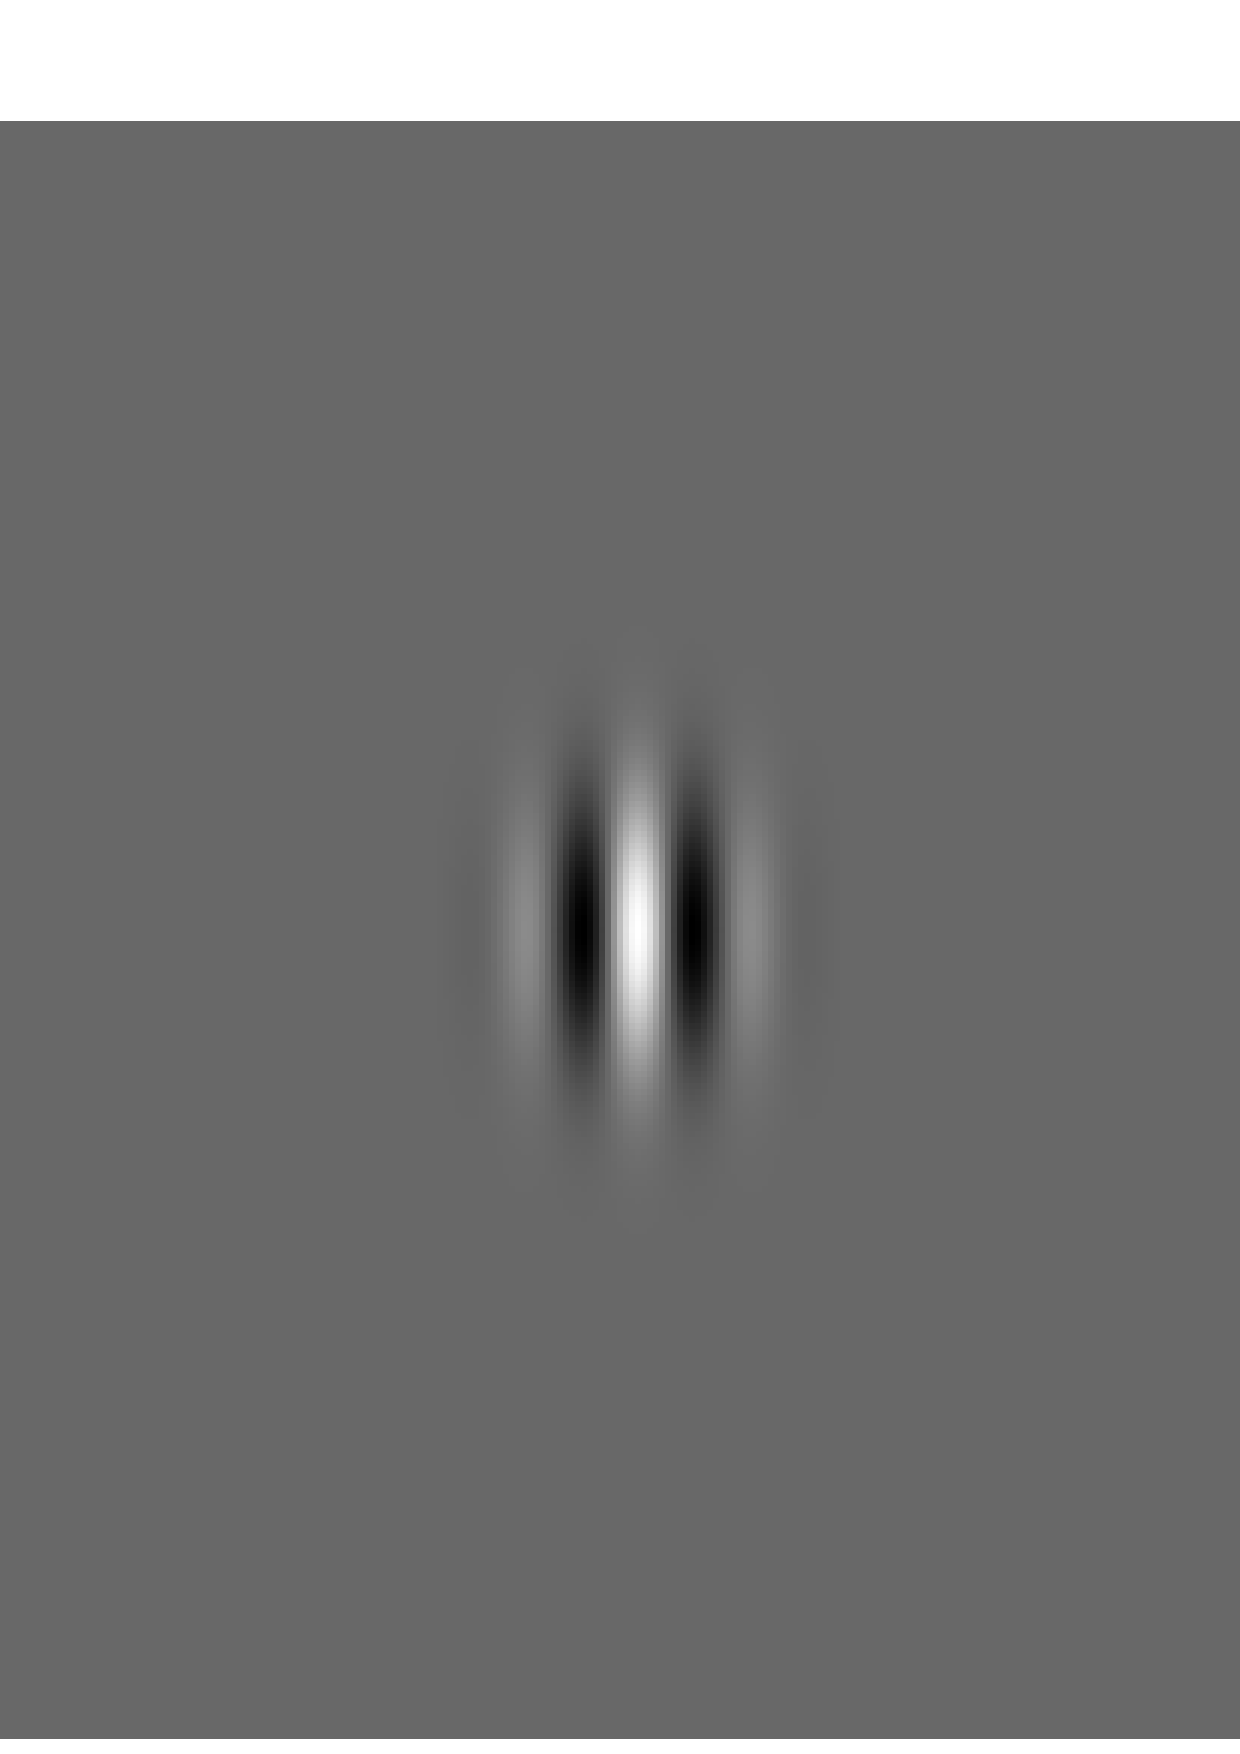
\includegraphics[scale=0.06]{Chapter3/Figures/Gabor-pi-2.png}}
\subfloat[$2\pi/3$]{

\includegraphics[scale=0.06]{Chapter3/Figures/Gabor-2pi-3.png}}
\subfloat[$5\pi/6$]{

\includegraphics[scale=0.06]{Chapter3/Figures/Gabor-5pi-6.png}}
\subfloat[$\pi$]{
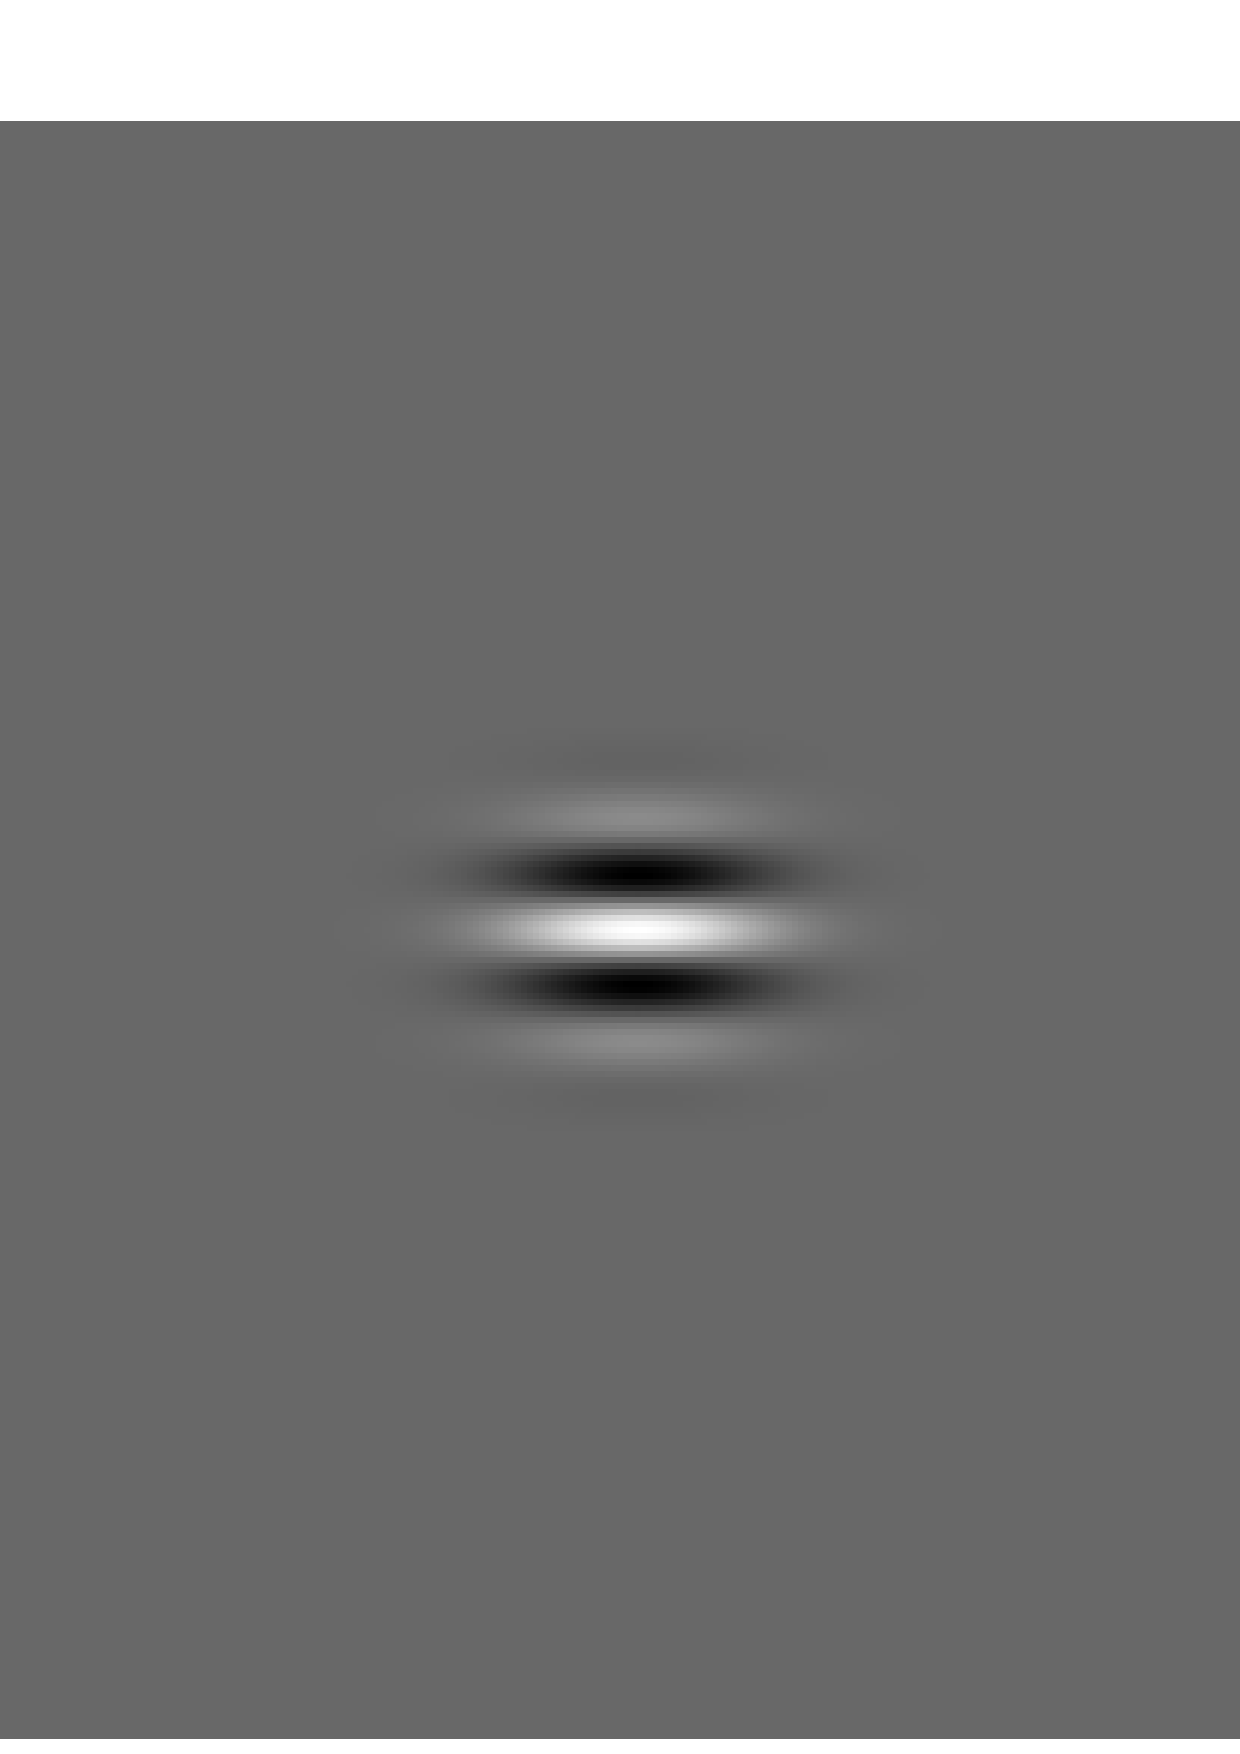
\includegraphics[scale=0.06]{Chapter3/Figures/Gabor-pi.png}}
\caption[Six orientation of Gabor filter]{The 6 orientations of the Gabor filters.}
\label{fig:GaborOrientation}
\end{figure}
		
The local patterns of the \ac{clbp} descriptor encode the magnitude and sign differences between the central pixel and its neighbors as well as the grey level of the central pixel rather than only the sign differences (general \ac{lbp}).
Figure \ref{fig:CLBPFig} represents this process.
The sign $CLBP_S$, magnitude $CLBP_M$, and central grey level $CLBP_C$ binary patterns are created by encoding the local distance components and the central grey levels.  

In the proposed framework, the rotation invariant, uniform, and normalized \ac{clbp} features with a radius of 3 and $24$ samples were calculated.
The radius and number of samples were chosen after testing the algorithm with different neighboring samples such as $\{8, 16, 24\}$ with a radius of $\{1,2,3\}$, respectively.
\end{description}
\begin{description}
\item[\acf{glcm} ($T_{2}$)] is one of the earliest texture descriptor methods, proposed by Haralick.~et al.~\cite{haralick1973textural}, widely used for texture analysis applications, including melanoma detection.
In this approach, texture features are extracted based on the statistical measurement of co-occurrence probabilities.
The co-occurrence distribution represents the occurrence probabilities of all the pairwise combinations of the grey levels in a defined window~\cite{clausi2002analysis}.
In other words, it counts how often a pixel with the grey intensity $i$ occurs adjacent to a pixel with the grey intensity $j$.
The spatial distance and orientation of interests between the pixels are defined by the distance $D$ and the angle $\theta$.
The co-occurrence probability between grey levels $i$ and $j$ is defined in Eq.~\ref{eq:GLCM}, where $P_{ij}$ represents the conditional probability of occurrences of the grey value $i$ adjacent to the grey value $j$ given the distance $D$ and orientation $\theta$.
Here, $G$ is the quantized number of grey levels:
\begin{equation}
    C_{ij} = \frac{P_{ij}}{\sum_{i,j=1}^{G} P_{ij}}.   
\label{eq:GLCM}
\end{equation}

The images are quantized to 32 grey levels and the co-occurrence probabilities are calculated given the distance ($D$) of 9 pixels and four different orientations of \{$\theta$ = $0^{\circ}$, $45^{\circ}$, $90^{\circ}$, $135^{\circ}$\}.
The final texture descriptor is an average of these four measurements allowing us to obtain a rotation invariant descriptor.
For each orientation, a set of 22 texture features (proposed in \cite{haralick1973textural, clausi2002analysis, soh1999texture}) are calculated.
These features are listed in Table~\ref{tab:glcmfeatures}
The proposed distance and quantization values were chosen after testing a variety of distances $\{1, 3, 7, 9\}$ and quantized grey-levels $\{16, 32, 64\}$.
%\begin{table}	
%\resizebox{0.9\textwidth}{0.49\textheight}{
%    \small{
%\begin{longtable}{|p{0.24\textwidth}|p{0.5\textwidth}}
	\begin{longtable}{lc}
	\caption[Extracted features by \ac{glcm} descriptor]{The list of \ac{glcm} statistics ($f_{1}$--$f_{22}$)~\cite{haralick1973textural,clausi2002analysis,soh1999texture} used in our experiments.
	The first section of the table represents the primary measures derived from the co-occurrence matrix $C_{ij}$ for calculating the features.
	Here, $\mu_{x}$, $\mu_{y}$, $\sigma_{x}$, and $\sigma_{y}$ are the mean and standard deviation of $C_{ij}$ with respect to $i$ and $j$, respectively.
	$H_{x}$ and $H_{y}$ are entropy of $C_{x}$ and $C_{y}$}\\
%\begin{center}	
	\toprule
	Co-occurrence matrix & $C_{ij} = P_{ij}/\sum_{i,j=1}^{G} P_{ij}$\\
	& \\[-0.8ex]	
	$C_{x}(i)$ & $\sum_{j=1}^{G}C_{ij}$\\
	& \\[-0.8ex]	
	$C_{y}(j)$ & $\sum_{i=1}^{G}C_{ij}$\\
	& \\[-0.8ex]	
	$C_{x+y}(k)$ & $\sum_{{ij}_{i+j=k}} C_{ij}, k = 2,3 , 2G$ \\
	& \\[-0.8ex]	
	$C_{x-y}(k)$ & $\sum_{{ij}_{|i-j|=k}} C_{ij}, k = 0,1 , G-1$ \\	
	& \\[-0.8ex]	
	$H_{xy}$ & $-\sum_{ij}C_{ij}\log C_{ij}$ \\	
	& \\[-0.8ex]	
	$H_{xy1}$ & $-\sum_{ij}C_{ij}\log(C_{x}(i)C_{y}(j))$\\
	& \\[-0.8ex]	
	$H_{xy2}$ & $-\sum_{ij}C_{x}(i)C_{y}(j)\log(C_{x}(i)C_{y}(j))$\\
	& \\[-0.8ex]	
	\hdashline	
	& \\[-0.8ex]		
	$f_{1}$: Maximum probability & $\max\{C_{ij} , \forall (ij)\}$ \\
	& \\[-0.8ex]
	$f_{2}$: Uniformity & $\sum_{ij} C_{ij}^{2}$ \\
	& \\[-0.8ex]
	$f_{3}$: Entropy & $\sum_{ij}C_{ij}\log C_{ij}$\\
	& \\[-0.8ex]
	$f_{4}$: Dissimilarity & $\sum_{ij} C_{ij}|i-j|$\\
	& \\[-0.8ex]
	$f_{5}$: Contrast & $\sum_{ij}C_{ij}|i-j|^{2}$ \\
	& \\[-1ex]
	$f_{6}$: Inverse difference & $\sum_{ij}C_{ij}/(1+|i-j|)$ \\
	&  \\[-1ex]
	$f_{7}$: Inverse difference moment & $\sum_{ij}C_{ij}/(1+|i-j|^{2})$ \\
	
%	\hline
%	\pagebreak
%	\hline
	& \\[-1ex]
	$f_{8}$: Correlation~1 & $\sum_{ij}(i-\mu_{x})(j-\mu_{y})C_{ij}/(\sigma_{x}\sigma_{y})$\\
	& \\[-1ex] 	
	$f_{9}$: Inverse difference normalized & $\sum_{ij}C_{ij}/(1+|i-j|/N)$\\
	& \\[-1ex]
	$f_{10}$: Sum of squares & $\sum_{ij} (i-\mu)^{2}C_{ij}$ \\
	& \\[-1ex]				
	$f_{11}$: Inverse difference moment normalized & $\sum_{ij}C_{ij}/(1+|i-j|^{2}/N^{2})$\\
	& \\[-1ex]
	$f_{12}$: Sum of average & $\sum_{i=1}^{2N-1}(i+1)C_{x+y}(i)$\\
	& \\[-1ex]
	$f_{13}$: Sum entropy & $S_{e} = -\sum_{i=1}^{2N-1}C_{x+y}(i)\log C_{x+y}(i)$\\
	& \\[-1ex]
	$f_{14}$: Sum variance & $\sum_{i=1}^{2N-1}(i+1-S_{e})^{2}C_{x+y}(i)$\\
	& \\[-1ex]
	$f_{15}$: Difference variance & $\sum_{i=1}^{2N-1}i^{2}C_{x-y}(i+1)$\\
	& \\[-1ex]
	$f_{16}$: Difference entropy & $-\sum_{i=1}^{2N-1} C_{x-y}(i+1)\log C_{x-y}(i)$\\
	& \\[-1ex]
	$f_{17}$: Information measure of correlation~1 & $H_{xy}-H_{xy1}/\max(H_{x},H_{y})$ \\
	& \\[-1ex]
	$f_{18}$: Information measure of correlation~2 & $\sqrt{1-e^{-2(H_{xy2}-H_{xy})}}$\\
	& \\[-1ex]
	$f_{19}$: Auto correlation & $C = \sum_{ij}ijC_{ij}$\\
	& \\[-1ex]	
%	\hline
%	\pagebreak
%	\hline
	$f_{20}$: Correlation~2 &  $(AC-\mu_{x}\mu_{y})/\sigma_{x}\sigma_{y}$ \\
	& \\[-1ex]	
	$f_{21}$: Cluster shade & $\sum_{ij} (i+j-\mu_{x}-\mu_{y})^{3}C_{ij}$\\
	& \\[-1ex]	
	$f_{22}$: Cluster prominence & $\sum_{ij} (i+j-\mu_{x}-\mu_{y})^{4}C_{ij}$\\
	\bottomrule
	\label{tab:glcmfeatures}
  	\end{longtable}
%}
%    }
%	\end{center}
%\label{Tab:glcmfeatures}
%\end{table}

\item[Gabor Filter ($T_{3}$)] is a linear filter which extracts edges and texture information from the image and was found to be similar to human visual perception~\cite{marvcelja1980mathematical}.
	The Gabor filter is defined as a modulation of a Gaussian kernel with a sinusoidal wave.
	The Gabor expression is shown in Eq.~\ref{eq:Gabor}.
	This function is basically a Gaussian with standard deviations of $\sigma_{x}$ and $\sigma_{y}$ that vary along the $x$ and $y$ axes while it is modulated by a complex sinusoidal with a wavelength of $\lambda$.
	In this equation, $\theta$ represents the orientation of the Gabor filter, $\psi$ is the phase offset, and $s$ is the scale factor.	
	\begin{subequations}
	\begin{align}
	g(x,y) & = \exp \left(-\left(\frac{x'^2}{2\sigma_{x}^{2}}+\frac{y'^{2}}{2\sigma_{y}^{2}}\right)\right) \cos\left(2\pi\frac{x'}{\lambda}+ \psi\right), \\
	x'& = s(x\cos\theta + y\sin\theta),\\
	y' &= s(-x\sin\theta + y\cos\theta).	
	\end{align}
	\label{eq:Gabor}
	\end{subequations}
	
In this work as described by \cite{Manjunath96-45}, the images are convolved with a set of Gabor filters characterized by different orientations and scales.
The features are created by considering the mean and variance of the resulting filtering.
We used 6 different orientations (\{$\pi/6$, $\pi/3$, $\pi/2$, $2\pi/3$, $5\pi/6$, $\pi$\}) along 4 scales, downsizing by a factor of two between each scale.
The first 6 filters are shown in Fig.~\ref{fig:GaborOrientation}.
%	\begin{figure}
	%\centering
	%\subfloat[$\pi/6$]{
	%
\includegraphics[scale=0.06]{Chapter3/Figures/Gabor-pi-6.png}}
	%\subfloat[$\pi/3$]{
	%
\includegraphics[scale=0.06]{Chapter3/Figures/Gabor-pi-3.png}}
	%\subfloat[$\pi/2$]{
	%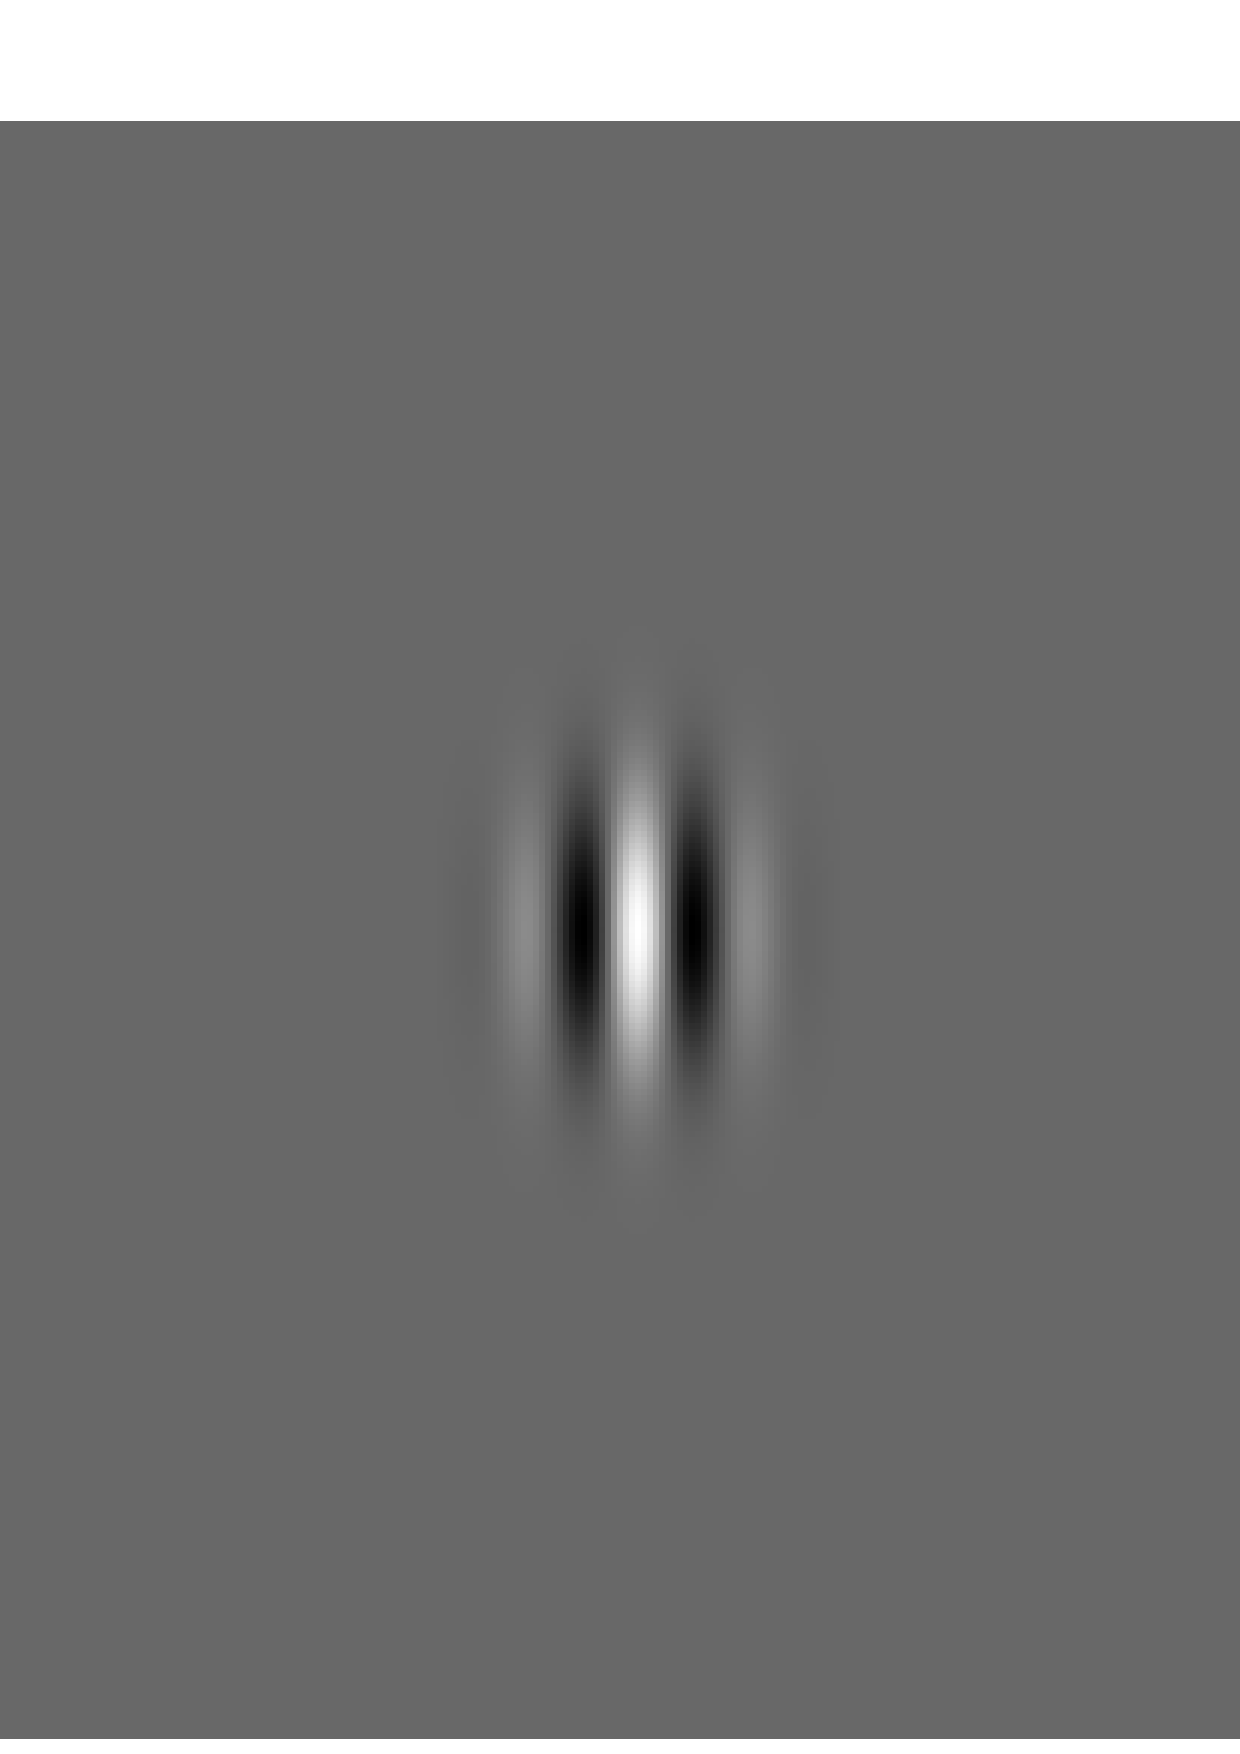
\includegraphics[scale=0.06]{Chapter3/Figures/Gabor-pi-2.png}}
	%\subfloat[$2\pi/3$]{
	%
\includegraphics[scale=0.06]{Chapter3/Figures/Gabor-2pi-3.png}}
	%\subfloat[$5\pi/6$]{
	%
\includegraphics[scale=0.06]{Chapter3/Figures/Gabor-5pi-6.png}}
	%\subfloat[$\pi$]{
	%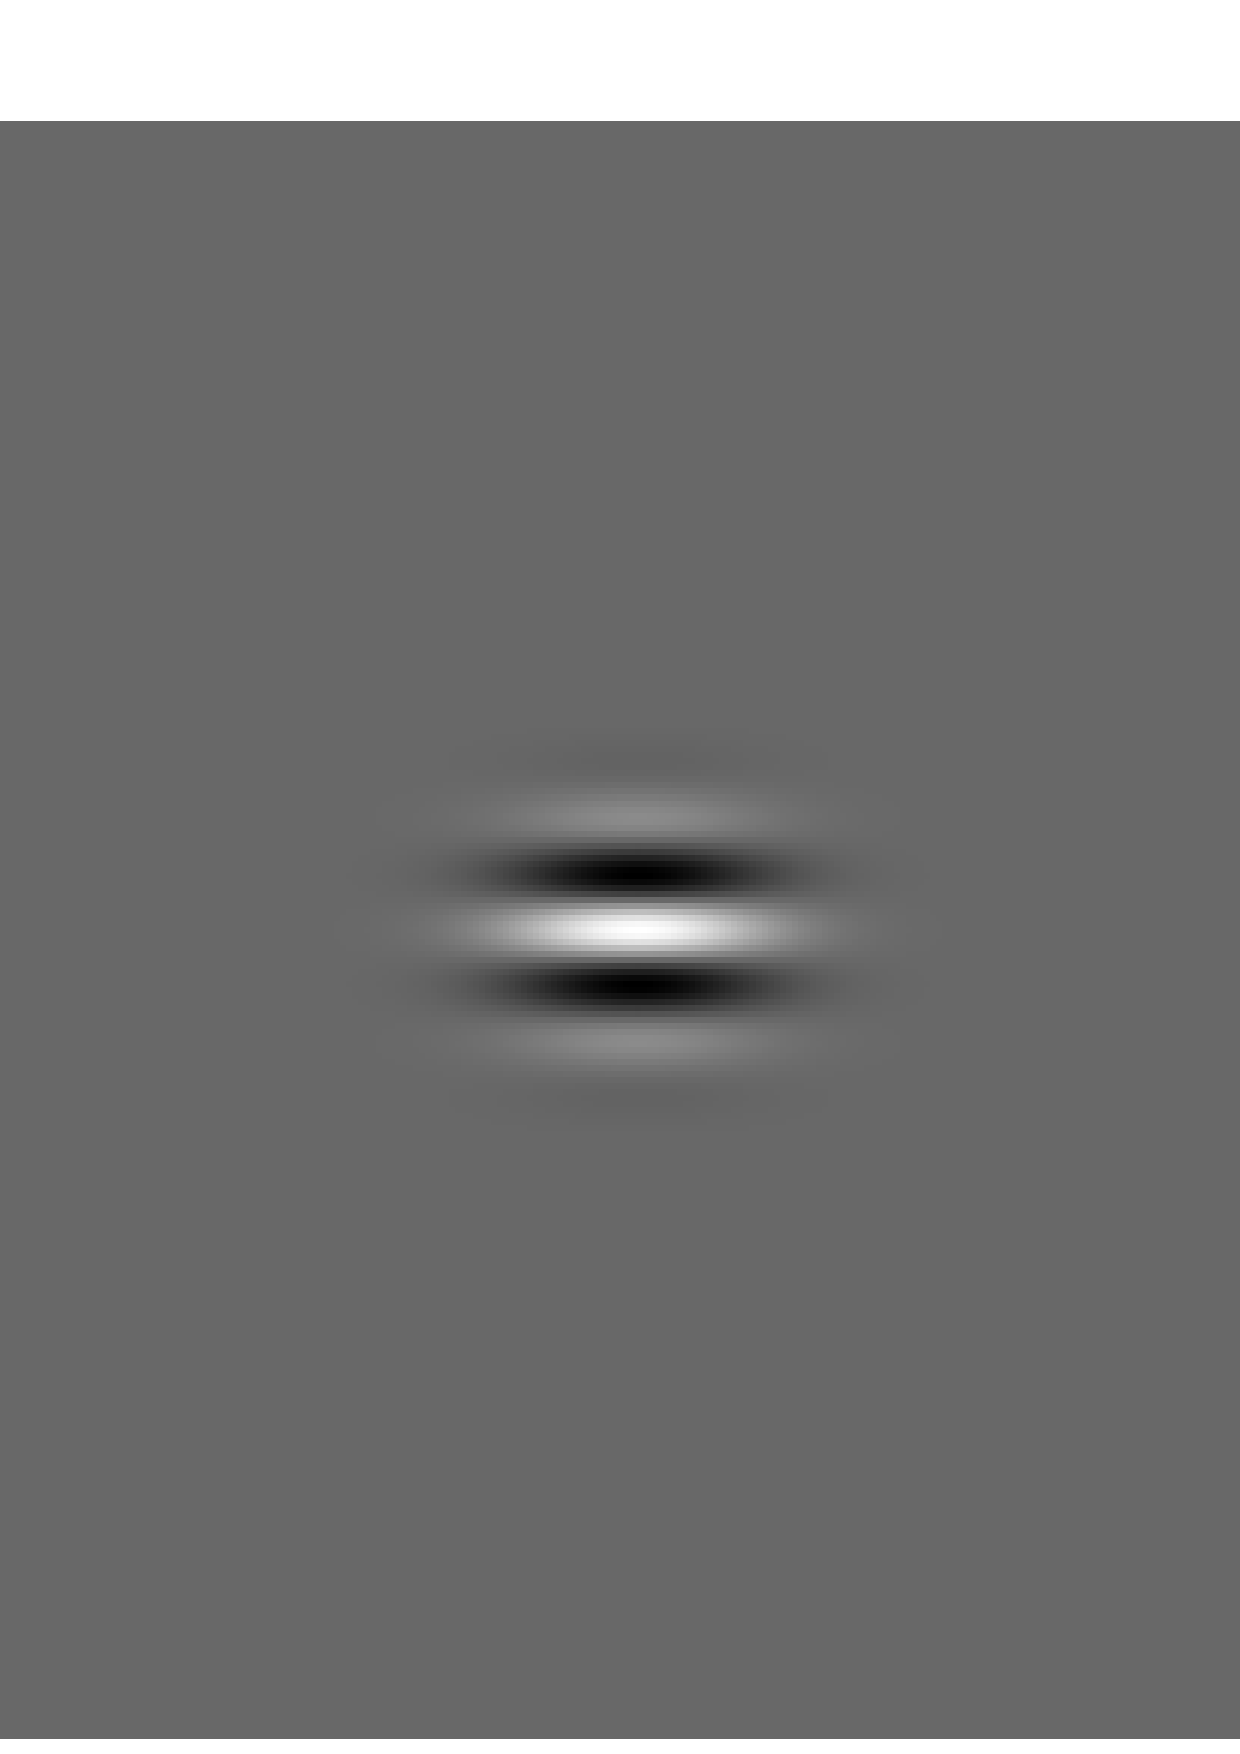
\includegraphics[scale=0.06]{Chapter3/Figures/Gabor-pi.png}}
	%\caption[Six orientations of the Gabor filter]{The 6 orientations of the Gabor filter.}
	%\label{fig:GaborOrientation}
	%\end{figure}

\item[\acf{hog} ($T_{4}$)] was proposed in \cite{dalal2005histograms}.
In simple terms, \ac{hog} counts the occurrences of gradient orientations in localized patches of an image.
This descriptor is invariant to geometric and photometric transformations.
\ac{hog} calculates the gradient values of the image by applying derivative filters ($[-1,0,1]$, $[-1,0,1]^{T}$) or the Sobel mask to the image and measuring the magnitude and orientations of the gradients.
Then, it creates the weighted histograms of the gradient orientations in the image patches.
The orientations are weighted either by the magnitude of gradients or by a function of gradient magnitudes.
In order to account for changes in illumination and contrast, the patches are grouped into larger spatially connected blocks and the final descriptor is formed by a vector of the normalized cell histograms from all the blocks.
	

\item[\acf{sift} ($T_{5}$)] proposed by Lowe et al.\cite{lowe2004distinctive} is a rotation, translation and scale invariant feature descriptor, used successfully by the computer vision society.
To identify the key-points, this descriptor first convolves the original image ($I(x,y)$) with Gaussian kernels ($G(x,y,k\sigma)$) at different scales ($k\sigma$).
\begin{equation}
L(x,y,k_{i}\sigma) = G(x,y,k_{i}\sigma)*I(x,y)~.
\label{eq:GaussianConv}
\end{equation}		
\noindent Then it creates the difference ($D$) of successive Gaussian blurred images (\acf{dog}) and identifies the key-points as the local maxima and minima of \ac{dog} images across the scales.
\begin{equation}
D(x,y,\sigma) = L(x,x, k_{i}\sigma) - L(x,x, k_{j}\sigma)~.
\label{eq:DoG}
\end{equation}
%Later it identifies the key-points as the local maxima and minima of \ac{dog} images across the scales.
\noindent Essentially each pixel in \ac{dog} images is compared with its 8 neighbor pixels at the same scale and 9 corresponding neighbor pixels in the neighboring scales.
This pixel is identified as the key-point if it has the maximum or minimum value among all its neighbors.
%	\begin{subequations}
%	\begin{align}
%		L(x,y,k_{i}\sigma) &= G(x,y,k_{i}\sigma)*I(x,y)~.\\
%	D(x,y,\sigma) &= L(x,x, k_{i}\sigma) - L(x,x, k_{j}\sigma)~.
%	\end{align}
%	\label{eq:DoG}
%	\end{subequations}
		   
In the next step, the identified key points are filtered to reject the ones with low contrast or those along the edges.
The remaining key points are then assigned one or more orientations based on the local image gradient directions.
In this step, the gradient magnitude and orientation of each neighboring pixel of the key point in the Gaussian blurred image $L$ is calculated.
For the sake of scale invariance, image $L(x,y)$ is selected at the same or closest scale ($\sigma$) of the key point of interest ($L(x,y,\sigma)$).
The gradient magnitude and orientation of all the neighboring pixels in image $L(x,y,\sigma)$ are computed as follows: 
\begin{subequations}
\begin{align}
m(x,y) & = \sqrt{(L(x+1,y) - L(x-1,y))^{2}+(L(x,y+1)-L(x,y-1))^{2}},\\
\theta(x,y) & = \tan^{-1}\left(\frac{L(x,y+1) - L(x,y-1)}{L(x+1,y) - L(x-1,y)}\right).
\end{align}
\end{subequations}
Then, using the computed magnitude and orientations of the pixels within a Gaussian circular weighted window $G_{L}$ around the key point, an orientation histogram is formed.
This histogram consists of 36-bins, each covering \ang{10}.
The orientation of each pixel in the neighborhood is accumulated to the histogram while weighted by its gradient magnitude and $G_{L}$.
Finally, the key point is assigned with the dominant orientation corresponding to the highest peak of the histogram as well as the local peaks within 80$\%$ of the highest one (up to two peaks in total). 
In this way, there can be several key points at the same location and scale but with different orientations.
The final key point descriptor is then created by taking a $16\times16$ neighborhood around the key point.
This neighborhood is divided into 16 sub-blocks of $4\times4$, and for each sub-block, an 8-bin orientation histogram is created.
Concatenation of these histograms (i.e. 16 regions) leads to a 128-dimensional feature vector as the final descriptor. 

\end{description}
